\documentclass[aspectratio=169,11pt]{beamer}

\usepackage{fontspec}
\usepackage{tikz}

\setsansfont{Arial}
\setmonofont{Consolas}

\definecolor{Navy}{HTML}{17324D}
\definecolor{Blue}{HTML}{2878B5}
\definecolor{Amber}{HTML}{D98B2B}
\definecolor{SoftBlue}{HTML}{EAF3F8}
\definecolor{Ink}{HTML}{243746}

\setbeamercolor{normal text}{fg=Ink,bg=white}
\setbeamercolor{frametitle}{fg=white,bg=Navy}
\setbeamerfont{frametitle}{series=\bfseries,size=\large}
\setbeamertemplate{navigation symbols}{}

\begin{document}

\begin{frame}{3. Thiết kế Data Warehouse đề xuất}
  \centering
  \vfill
  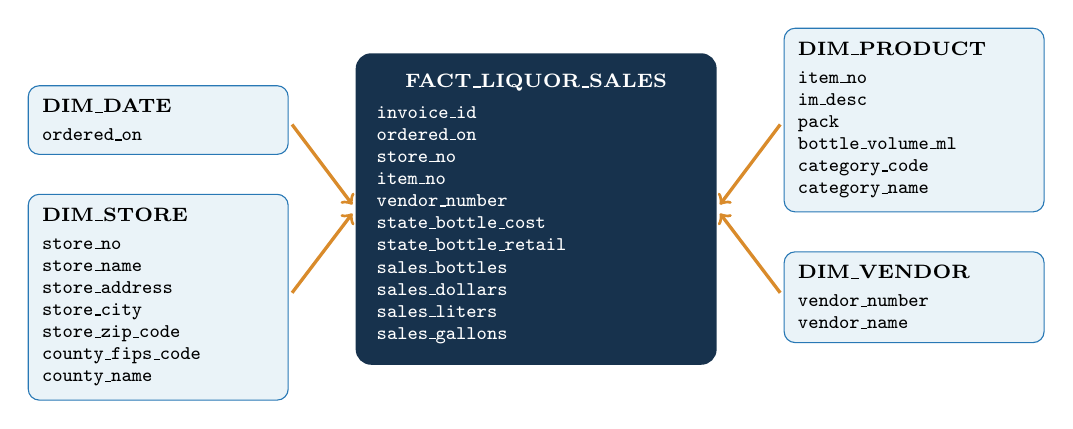
\begin{tikzpicture}[
    x=1cm,y=1cm,
    dim/.style={draw=Blue, fill=SoftBlue, rounded corners=4pt,
      minimum width=3.25cm, text width=2.95cm, inner sep=5pt,
      align=left, font=\scriptsize},
    fact/.style={draw=Navy, very thick, fill=Navy, text=white,
      rounded corners=5pt, minimum width=4.35cm, text width=4.05cm,
      inner sep=7pt, align=left, font=\scriptsize},
    link/.style={->, very thick, color=Amber, shorten >=2pt, shorten <=2pt}
  ]
    \node[dim] (date) at (1.75,3.35) {
      \textbf{DIM\_DATE}\par\vspace{2pt}
      \texttt{ordered\_on}
    };

    \node[dim] (store) at (1.75,1.10) {
      \textbf{DIM\_STORE}\par\vspace{2pt}
      \texttt{store\_no}\par
      \texttt{store\_name}\par
      \texttt{store\_address}\par
      \texttt{store\_city}\par
      \texttt{store\_zip\_code}\par
      \texttt{county\_fips\_code}\par
      \texttt{county\_name}
    };

    \node[fact] (fact) at (6.55,2.22) {
      \centering\textbf{FACT\_LIQUOR\_SALES}\par\vspace{3pt}
      \raggedright
      \texttt{invoice\_id}\par
      \texttt{ordered\_on}\par
      \texttt{store\_no}\par
      \texttt{item\_no}\par
      \texttt{vendor\_number}\par
      \texttt{state\_bottle\_cost}\par
      \texttt{state\_bottle\_retail}\par
      \texttt{sales\_bottles}\par
      \texttt{sales\_dollars}\par
      \texttt{sales\_liters}\par
      \texttt{sales\_gallons}
    };

    \node[dim] (product) at (11.35,3.35) {
      \textbf{DIM\_PRODUCT}\par\vspace{2pt}
      \texttt{item\_no}\par
      \texttt{im\_desc}\par
      \texttt{pack}\par
      \texttt{bottle\_volume\_ml}\par
      \texttt{category\_code}\par
      \texttt{category\_name}
    };

    \node[dim] (vendor) at (11.35,1.10) {
      \textbf{DIM\_VENDOR}\par\vspace{2pt}
      \texttt{vendor\_number}\par
      \texttt{vendor\_name}
    };

    \draw[link] (date.east) -- (fact.west);
    \draw[link] (store.east) -- (fact.west);
    \draw[link] (product.west) -- (fact.east);
    \draw[link] (vendor.west) -- (fact.east);
  \end{tikzpicture}
  \vfill
\end{frame}

\end{document}
